\documentclass[{../../master}]{subfiles}
\graphicspath{{../..}}  % 個別コンパイル時の画像パスを解決する

\begin{document}

\section{背景}

社会実装指向型研究では,研究成果を現場へ持ち込み,ユーザのレビューから改善点を即座にフィードバックするアジャイル型開発のアプローチが要求されます.
しかし,ロボット等のメカニカルデバイスを必要とする研究テーマでは,デバイスの設計開発に多くの時間を必要とすることから,アジャイル型開発が適用しにくい状況がありました.

この課題に対し,一関高専では,東京高専・和歌山高専と共同で自律移動ロボットプラットフォームの開発に取り組んでいます.
これは,自律移動に関する部分をプラットフォーム化して提供することで,目的の機能の開発に注力できることを目標としたものです.
これまでの研究で,図\ref{fig:previous_work}に示すような大径インホイールモータを搭載した移動ロボットが開発されました.

\begin{figure}[h]
  \centering
  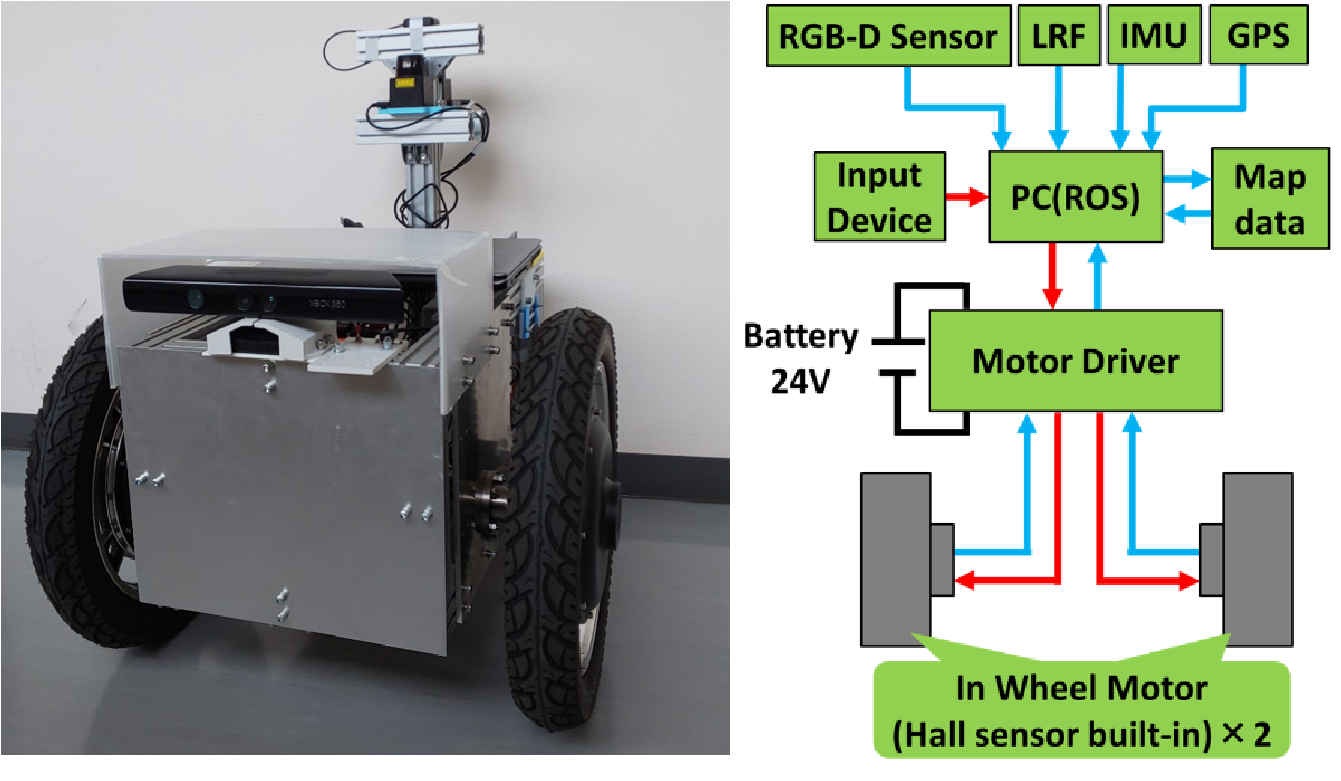
\includegraphics[width=80truemm, clip]{images/previous_work.pdf}
  \caption{Appearance and System Configuration of The Mobile Robot Platform Developed so far}
  \label{fig:previous_work}
\end{figure}

\end{document}